% ==================== 文档类与编码 ====================
\documentclass[UTF8,a4paper,12pt]{ctexart}

% ==================== 页面与版式 ====================
\usepackage[a4paper,margin=2.5cm]{geometry}
\usepackage{setspace}
\onehalfspacing
\setlength{\parskip}{0.5em}

% ==================== 数学公式 ====================
\usepackage{amsmath,amssymb}

% ==================== 图片 ====================
\usepackage{graphicx}
\graphicspath{{figures/}}   % 图片放在 figures/ 文件夹下
\usepackage{float}          % 支持 [H] 强制固定图片位置

% ==================== 表格 ====================
\usepackage{booktabs}
\usepackage{array}

% ==================== 代码高亮 ====================
\usepackage{listings}
\usepackage{xcolor}

\lstset{
  basicstyle=\ttfamily\small,
  keywordstyle=\color{blue!70},
  commentstyle=\color{green!50!black},
  stringstyle=\color{orange},
  numbers=left,
  numberstyle=\tiny\color{gray},
  stepnumber=1,
  frame=single,
  breaklines=true,
  captionpos=b,
  showstringspaces=false
}

\lstdefinestyle{terminal}{
  language=bash,
  basicstyle=\ttfamily\small\color{green!80!black},
  backgroundcolor=\color{black!85},
  keywordstyle=\color{cyan},
  commentstyle=\color{gray},
  stringstyle=\color{yellow},
  numbers=none,
  frame=single,
  frameround=tttt,
  rulecolor=\color{gray!30},
  breaklines=true
}

% ==================== 页眉页脚 ====================
\usepackage{fancyhdr}
\setlength{\headheight}{14pt}
\pagestyle{fancy}
\fancyhf{}
\fancyfoot[C]{第~\thepage~页}
\renewcommand{\headrulewidth}{0pt}
\renewcommand{\footrulewidth}{0pt}

% ==================== 目录样式 ====================
\usepackage{titletoc}
\titlecontents{section}
  [0em]
  {\addvspace{0.5ex}\bfseries}
  {\contentslabel{1.8em}}
  {}
  {\titlerule*[0.5pc]{.}\contentspage}

% ==================== 标题信息（每次改这里） ====================
\title{\Large\bfseries 金融大数据处理技术-实验2}
\author{黎俊 \\ 241275043}
\date{2026年10月25日}

% ==================== 正文开始 ====================
\begin{document}

% ==================== 封面（无页码） ====================
\maketitle
\thispagestyle{empty}

% ==================== 目录页（有页码） ====================
\clearpage
\pagenumbering{arabic}
\tableofcontents
\thispagestyle{fancy}

% ==================== 正文开始 ====================
\clearpage

% ============================================================
% 第 1 章 实验概述
% ============================================================
\section{实验概述}

\subsection{实验目的}

本实验基于 Hadoop MapReduce 分布式计算框架，对银行脱敏信贷客户数据进行统计分析
与建模预测。实验共 5 个任务：任务 1--4 对原始客户数据做特征工程层面的预处理与统计
探索分析，挖掘客户资产分布、分群特征；任务 5 在前期分析基础上利用 MapReduce 实现
客户信贷风险预测模型，理解分布式计算框架下机器学习预测任务的实现思路。

通过本实验重点掌握 MapReduce 编程范式，学习分布式缓存（DistributedCache）、
Mapper/Reducer 分工、任务调度、模型加载与分布式预测等核心知识。

\subsection{实验环境}

\begin{table}[H]
  \centering
  \caption{实验环境配置}
  \label{tab:env}
  \begin{tabular}{lcc}
    \toprule
    组件 & 版本 & 说明 \\
    \midrule
    OS & Ubuntu & 64 位 \\
    Java & OpenJDK 11 & Hadoop 3.x 要求 \\
    Hadoop & 3.5.0 & 单机伪分布式 \\
    Maven & 3.9.9 & 项目构建 \\
    \bottomrule
  \end{tabular}
\end{table}

\subsection{数据集}

数据来源为脱敏后的银行信贷客户数据，原始数据含 627 个字段，经筛选保留 15 个有效字段，
分为训练集 \texttt{train.csv} 与测试集 \texttt{test.csv}。任务 1--4 只使用
\texttt{train.csv}，任务 5 同时使用两个数据集。主要字段如下：

\begin{table}[H]
  \centering
  \caption{主要字段说明}
  \label{tab:fields}
  \begin{tabular}{lll}
    \toprule
    列名 & 类型 & 含义 \\
    \midrule
    CUST\_ID & bigint & 客户唯一标识 ID \\
    OPEN\_ORG\_NUM & bigint & 开户机构编号 \\
    bad\_good & bigint & 客户好坏标签（0/1） \\
    CUST\_SAVING\_AMT $\sim$ CUST\_METAL\_AMT & double & 存款、理财、私人理财、基金、国债、银保通、贵金属 7 类资产 \\
    CUST\_ASSET\_AMT & double & 资产总额 \\
    CUST\_DEBT\_AMT & double & 负债总额 \\
    G\_OS\_PRCP\_SUM & double & 贷款账户月余额 \\
    LOAN\_FLAG / CRED\_FLAG & string & 个贷标识 / 持有基金标志 \\
    \bottomrule
  \end{tabular}
\end{table}

其中训练集含 285285 条记录（好客户 280401，坏客户 4884），测试集含 189766 条记录
（无标签）。

% ============================================================
% 第 2 章 设计思路
% ============================================================
\section{设计思路}

各任务分别实现为独立的 Driver 类，共享 \texttt{Csv.java} 中的 CSV 解析辅助方法：
缺失值 / 非法数值统一按 0 处理，表头通过首列是否为 \texttt{CUST\_ID} 识别。

\subsection{任务 1：各开户机构客户数量及资产统计}

\begin{itemize}
  \item \textbf{Mapper}：逐行解析 \texttt{train.csv}，以 \texttt{OPEN\_ORG\_NUM}
        为 key，value 组合为 \texttt{1 <TAB> 资产 <TAB> 负债 <TAB> 是否逾期}；
  \item \textbf{Reducer}：按机构累加客户数、总资产、总负债、逾期客户数
        （\texttt{bad\_good == 1}）。
\end{itemize}

输出格式：\texttt{机构编号 <TAB> 客户数量,总资产,总负债,个贷逾期客户数}。

\subsection{任务 2：平均值分析}

实现为两阶段流水线：

\begin{enumerate}
  \item \textbf{Job A（map-only，单 reducer）}：读取任务 1 输出，计算每个机构的
        平均资产（总资产 / 客户数量），写入中间目录；
  \item \textbf{Job B}：通过 \texttt{addCacheFile} 将平均值表加入
        DistributedCache，Mapper 在 \texttt{setup()} 中加载为
        \texttt{Map<机构, 平均资产>}，遍历 \texttt{train.csv} 逐客户比较资产与
        机构平均值（等于平均值归入“高于”部分），Reducer 统计高于/低于数量。
\end{enumerate}

\subsection{任务 3：客户总资产四分位数}

利用 MapReduce 框架内置的排序机制：Map 以 \texttt{CUST\_ASSET\_AMT} 为 key 输出，
经 Shuffle（分区、排序）后进入单个 Reducer（\texttt{setNumReduceTasks(1)}），
获得全局升序的资产序列；再结合总样本条数用线性插值法计算四分位数：

\[
\mathrm{pos} = p \cdot (n - 1), \qquad
Q_p = x_{\lfloor \mathrm{pos} \rfloor}
      + (\mathrm{pos} - \lfloor \mathrm{pos} \rfloor)
        \cdot (x_{\lceil \mathrm{pos} \rceil} - x_{\lfloor \mathrm{pos} \rfloor})
\]

该插值方式等价于 numpy 默认的 \texttt{linear} 插值。

\subsection{任务 4：客户资产分层与资产结构统计}

\begin{itemize}
  \item \textbf{阈值注入}：Driver 先从任务 3 输出中解析 Q25/Q50/Q75，通过
        \texttt{Configuration.setDouble} 注入作业；
  \item \textbf{分层}：Mapper 按资产与四分位数的关系把客户划分为 低资产 / 中等资产 /
        较高资产 / 高资产 四层（tier 0--3），并对每层发射 7 类资产的金额；
  \item \textbf{聚合与排序}：Reducer 汇总每类资产金额后计算占比，先按层级升序
        （单 reducer 保证顺序集中），层内按占比降序排序输出。
\end{itemize}

\subsection{任务 5：客户信贷风险预测（高斯朴素贝叶斯）}

选用高斯朴素贝叶斯（Gaussian Naive Bayes）作为分类器，实现为“训练 + 预测”两个 Job：

\begin{enumerate}
  \item \textbf{训练 Job}：TrainMapper 发射类别先验频度（key = \texttt{C<TAB>label}）
        与每类每特征的 \texttt{1<TAB>x<TAB>x$^2$}（key = \texttt{F<TAB>label<TAB>j}）；
        TrainReducer 汇总得到每类先验、均值、方差，输出紧凑模型文件（单 reducer）。
  \item \textbf{预测 Job（map-only）}：模型经 DistributedCache 分发，PredictMapper
        在 \texttt{setup()} 中加载模型，对每个测试样本计算两类的对数后验概率并取
        最大类别：
\end{enumerate}

\[
\hat{y} = \arg\max_{c} \left[
  \ln P(c) + \sum_{j=1}^{d} \ln \mathcal{N}(x_j; \mu_{c,j}, \sigma^2_{c,j})
\right]
\]

针对训练集中某类下恒定特征（方差 $\approx 0$，例如坏样本的 \texttt{G\_OS\_PRCP\_SUM}
全为 0）会被高斯分布过度加权的问题，在 \texttt{setup()} 中对每个特征方差加入“该特征
全局方差（组内 + 组间）的 1\%”作为加性平滑项，避免单一零方差特征主导预测结果。

% ============================================================
% 第 3 章 运行结果
% ============================================================
\section{运行结果}

全部作业在单机伪分布式集群上运行成功，共 7 个 MapReduce Job（任务 1、任务 3、
任务 4 各 1 个，任务 2、任务 5 各 2 个）均为 SUCCEEDED 状态（见附录截图）。

\subsection{任务 1 结果}

共统计 687 个开户机构，节选如下（金额保留两位小数）：

\begin{table}[H]
  \centering
  \caption{任务 1 结果节选}
  \label{tab:t1}
  \begin{tabular}{lcccc}
    \toprule
    机构编号 & 客户数量 & 总资产 & 总负债 & 逾期客户数 \\
    \midrule
    1001 & 1254 & 184485852.19 & 112193577.37 & 32 \\
    1002 & 793  & 85762009.43  & 28727466.60  & 5  \\
    1003 & 887  & 116772867.93 & 23132764.24  & 9  \\
    101  & 1241 & 293699077.32 & 131735191.75 & 54 \\
    \bottomrule
  \end{tabular}
\end{table}

机构 1001：1254 个客户，总资产 184485852.19，总负债 112193577.37，逾期客户数 32
（即 \texttt{bad\_good==1} 的客户数，经 \texttt{awk} 校验）。

\subsection{任务 2 结果}

共 687 个机构，节选如下：

\begin{table}[H]
  \centering
  \caption{任务 2 结果节选}
  \label{tab:t2}
  \begin{tabular}{lcc}
    \toprule
    机构编号 & 高于平均资产客户数 & 低于平均资产客户数 \\
    \midrule
    1001 & 232 & 1022 \\
    1002 & 106 & 687  \\
    1003 & 144 & 743  \\
    101  & 203 & 1038 \\
    \bottomrule
  \end{tabular}
\end{table}

机构 1001 结果 \texttt{232,1022} 与示例一致。

\subsection{任务 3 结果}

四分位数输出（单行）：

\begin{lstlisting}[style=terminal]
Q25:1127.35   Q50:6501.38   Q75:49173.11
\end{lstlisting}

经 Python（numpy 线性插值）交叉验证一致。

\subsection{任务 4 结果}

共 28 行（4 层 $\times$ 7 类资产），完整结果如下：

\begin{table}[H]
  \centering
  \caption{任务 4：各资产层级资产结构占比}
  \label{tab:t4}
  \begin{tabular}{lll}
    \toprule
    等级 & 资产种类 & 占比 \\
    \midrule
    低资产   & 存款   & 0.9963 \\
    低资产   & 基金   & 0.0027 \\
    低资产   & 贵金属 & 0.0009 \\
    低资产   & 银保通 & 0.0001 \\
    低资产   & 国债   & 0.0000 \\
    低资产   & 理财   & 0.0000 \\
    低资产   & 私人理财 & 0.0000 \\
    中等资产 & 存款   & 0.9858 \\
    中等资产 & 基金   & 0.0102 \\
    中等资产 & 银保通 & 0.0029 \\
    中等资产 & 贵金属 & 0.0007 \\
    中等资产 & 国债   & 0.0003 \\
    中等资产 & 理财   & 0.0001 \\
    中等资产 & 私人理财 & 0.0000 \\
    较高资产 & 存款   & 0.9567 \\
    较高资产 & 基金   & 0.0267 \\
    较高资产 & 理财   & 0.0064 \\
    较高资产 & 银保通 & 0.0062 \\
    较高资产 & 国债   & 0.0032 \\
    较高资产 & 贵金属 & 0.0009 \\
    较高资产 & 私人理财 & 0.0000 \\
    高资产   & 存款   & 0.5602 \\
    高资产   & 理财   & 0.2949 \\
    高资产   & 私人理财 & 0.1086 \\
    高资产   & 基金   & 0.0265 \\
    高资产   & 国债   & 0.0083 \\
    高资产   & 银保通 & 0.0013 \\
    高资产   & 贵金属 & 0.0003 \\
    \bottomrule
  \end{tabular}
\end{table}

其中“中等资产 $\rightarrow$ 存款 $\rightarrow$ 0.9858”与示例一致。可以看出：低/中等
资产客户以存款为主（占比 $> 98\%$），高资产客户资产配置显著多元化（理财 + 私人理财
占比约 40\%）。

\subsection{任务 5 结果}

对 189766 个测试客户完成预测，节选如下：

\begin{lstlisting}[style=terminal]
1000000239  0
1000003260  0
1000003414  0
1000007147  1
...
\end{lstlisting}

预测分布：预测为 0（好客户）184759 个，预测为 1（坏客户）5007 个，坏客户比例约
2.64\%，与训练集先验（坏客户约 1.71\%）基本一致，模型无退化。模型核心目标是掌握
MapReduce 分布式预测流程，分数不作为重点。

% ============================================================
% 第 4 章 可能的改进之处
% ============================================================
\section{可能的改进之处}

\begin{enumerate}
  \item \textbf{去重 / 局部预聚合}：任务 1 中每个客户产生 1 条、任务 4 中每个客户
        产生 7 条中间记录，可添加 Combiner 在 Map 端先局部求和，显著减少 shuffle
        数据量。
  \item \textbf{任务 3 单 Reducer 内存风险}：四分位数计算依赖单 reducer 把全部资产
        加载进内存，数据量极大时可能 OOM，可改用近似分位数（如 t-digest）或多
        reducer + 分桶汇总的方式。
  \item \textbf{任务 4 依赖读取方式}：当前 Driver 用 \texttt{FileSystem.open} 读取
        任务 3 输出解析四分位数，可改用 DistributedCache 替代，使依赖关系在任务调度
        层面更规范。
  \item \textbf{模型扩展性}：任务 5 目前为单 reducer 训练、内存加载模型，可扩展到
        多类别、加入特征选择 / 标准化；朴素贝叶斯假设特征独立，可尝试引入特征相关性
        处理或改用其他分类器。
  \item \textbf{参数化与配置化}：特征索引、机构字段、输出格式等目前硬编码，可外置到
        配置文件或作业参数，便于复用。
\end{enumerate}

% ============================================================
% 附录：运行截图
% ============================================================
\section*{附录：运行成功的 Web 页面截图}
\addcontentsline{toc}{section}{附录：运行成功的 Web 页面截图}

\begin{figure}[H]
  \centering
  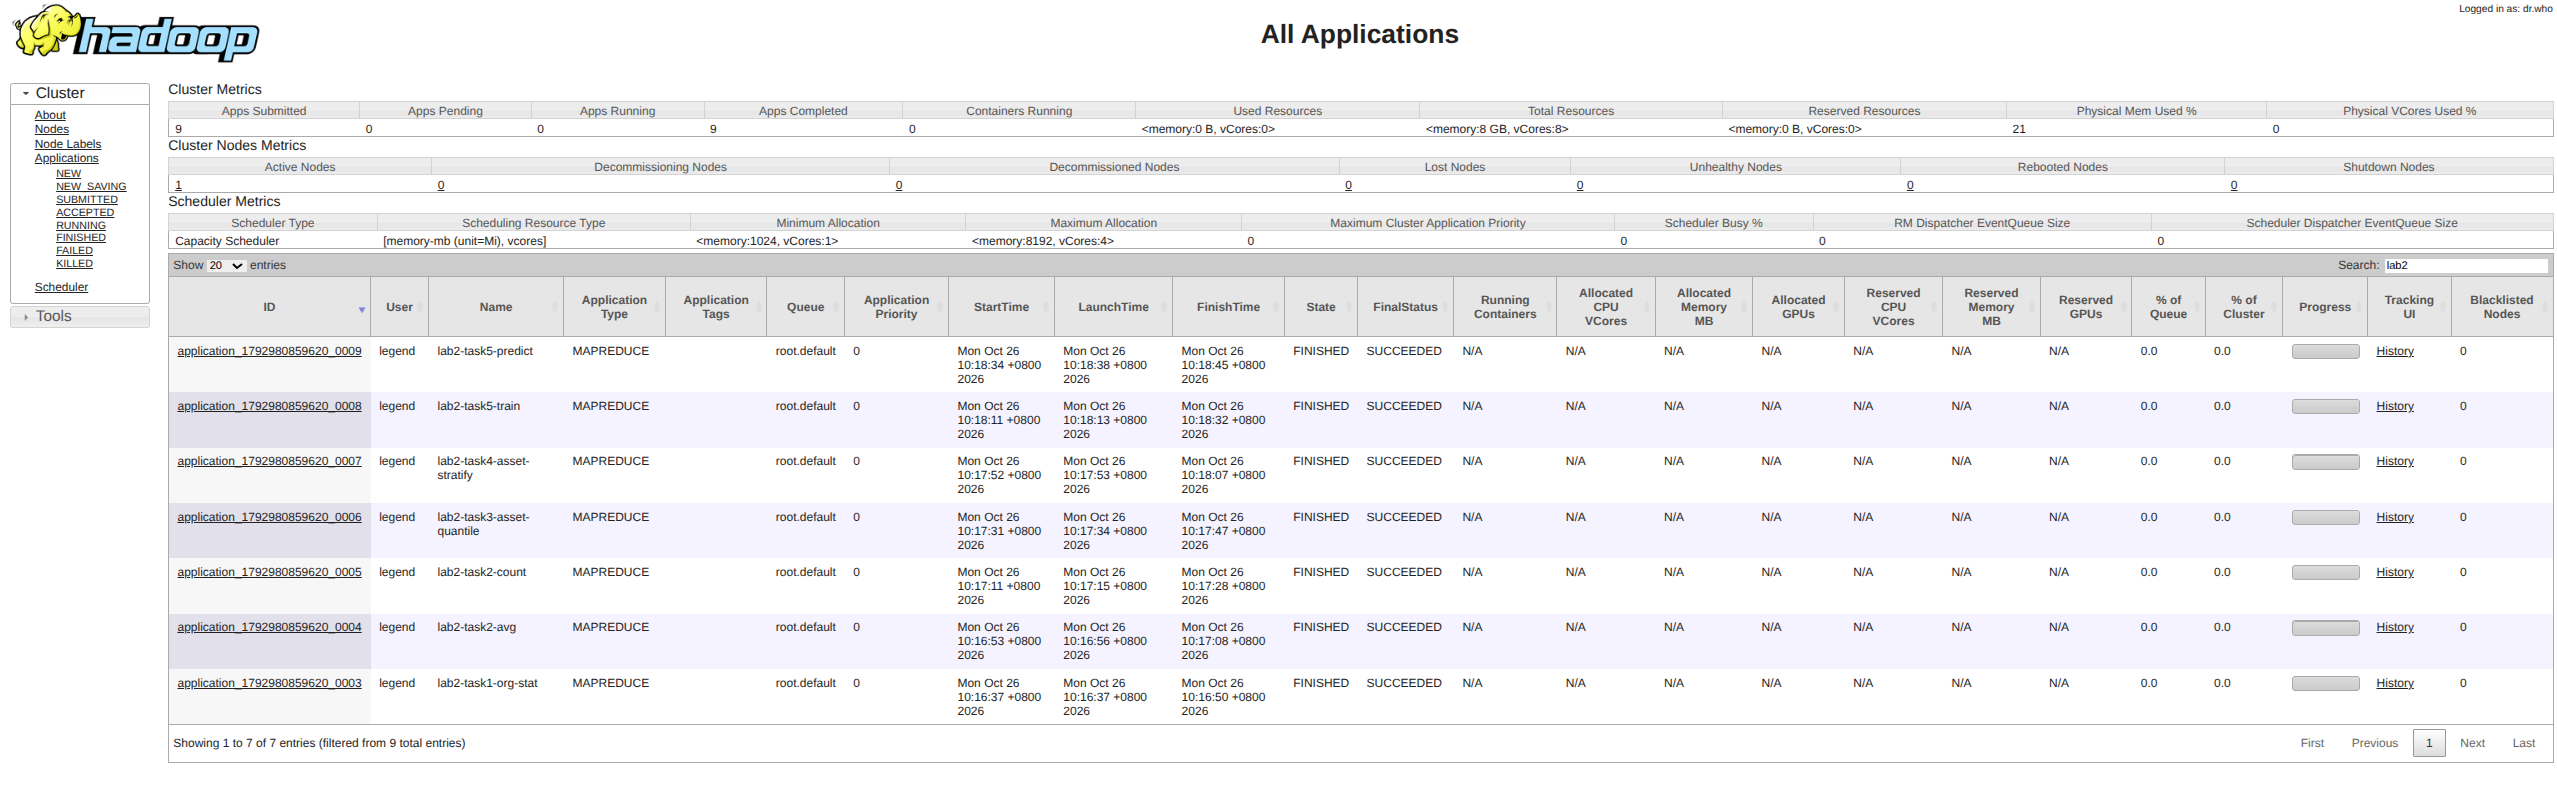
\includegraphics[width=1.0\textwidth]{yarn_web.png}
  \caption{YARN ResourceManager 运行成功截图（全部作业 SUCCEEDED）}
  \label{fig:yarn}
\end{figure}

\end{document}
